% \ssec{Data pipeline on premises}
% \begin{frame}{Data pipeline on premises}
% 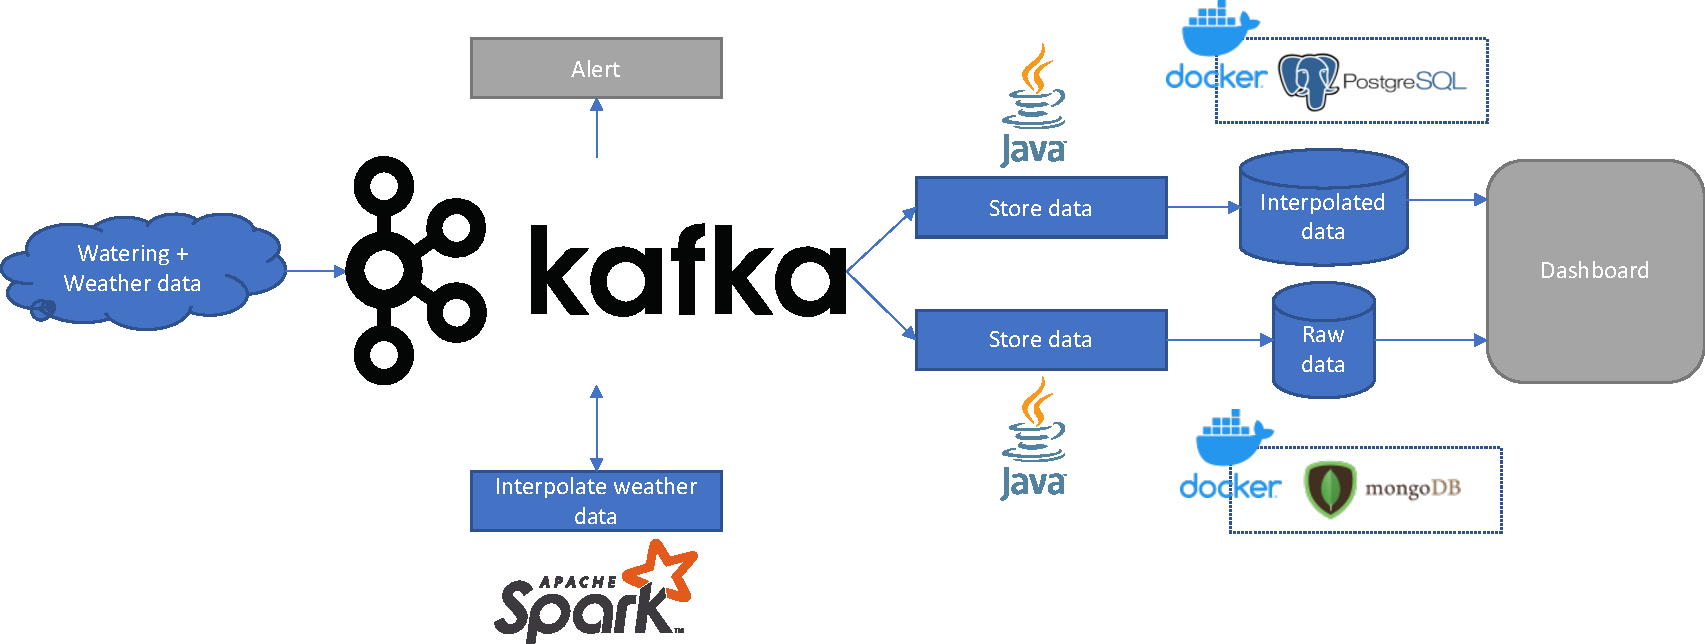
\includegraphics[width=\linewidth]{imgs/pipeline_prem.pdf}
% \end{frame}

\sec{Data pipeline on AWS}

\begin{frame}[allowframebreaks]{AWS}
Useful links and sources
\begin{table}[]
    \centering
    \footnotesize
    \begin{tabular}{ll}
        \textbf{Resource} & \textbf{Link} \\\hline
        AWS Educate & \url{https://aws.amazon.com/it/education/awseducate/}\\
        AWS Console & \url{https://console.aws.amazon.com/console/home?region=us-east-1}\\
        IAM & \url{https://docs.aws.amazon.com/IAM/latest/UserGuide/iam-ug.pdf}\\
        SDK & \url{https://docs.aws.amazon.com/sdk-for-java/latest/developer-guide/home.html}\\
        Lambda & \url{https://docs.aws.amazon.com/lambda/latest/dg/getting-started.html}\\
               & \url{https://console.aws.amazon.com/lambda/home?region=us-east-1\#/functions}\\
        Kinesis & \url{https://docs.aws.amazon.com/streams/latest/dev/introduction.html}\\
        DynamoDB & \url{https://docs.aws.amazon.com/amazondynamodb/latest/developerguide/Introduction.html}\\
    \end{tabular}
\end{table}

Amazon Web Services (AWS) is a platform of web services
\i computing, storing, and networking, at different abstraction layers 
\i web service means services controlled via a (visual) web interface
\i EC2, which offers virtual servers, and S3, which offers storage capacity
\si E.g., Linux server with an optimized distribution
called Amazon Linux
\si Virtual servers can fail, so you need at least two of them
\si The load balancer will distribute the traffic between them
    
Clouds are often divided into types
\i Public, public usage
\i Private, private usage
\i Hybrid, a mixture of a public and a private cloud
AWS is a public cloud

Cloud computing services also have several classifications:
\i Infrastructure as a service (IaaS)
\si fundamental resources like computing,
storage, and networking
\i Platform as a service (PaaS)
\si deploy applications to
cloud platforms (AWS Elastic Beanstalk, Heroku)
\i Software as a service (SaaS)
\si provide software running in
the cloud (Amazon WorkSpaces, and Microsoft Office 365)

AWS product portfolio contains IaaS, PaaS, and SaaS
\end{frame}

\begin{frame}[allowframebreaks]{Accessing the cloud}
Most cloud services can be accessed in multiple ways. First, most
support access via the web, thus permitting intuitive point and click
access without any programming or even local software installation
(beyond a web browser) on your part. The availability of such
intuitive interfaces is part of the attraction of cloud services.

A web interface becomes tedious if the same or similar actions
must be performed repeatedly. In such cases, you likely want to
write programs that issue requests to cloud services on your behalf.
Fortunately, most cloud services support such programmatic access.
Typically, they support a Representational State Transfer (REST)
application programming interface (API) that permits requests to be
transmitted via the secure Hypertext Transfer Protocol (HTTPS) that
is used by web browsers. (This common use of HTTPS is not a
coincidence: the web interfaces discussed in the first paragraph are
often implemented via browser-hosted Javascript programs that
generate such REST messages.) REST APIs are the key to
programmatic interactions with cloud services.

One way to interact with cloud services programmatically is to
write programs that generate REST messages directly. However,
while constructing REST messages “by hand” may appeal to hardcore
system programmers, you will normally want to access cloud
services via software development kits (SDKs) that you install on
your computer. Such SDKs permit access from programming
languages such as Python (our choice in this book), C++, Go, Java,
PHP, and Ruby.
\end{frame}


\begin{frame}{Interacting with AWS}

\i Management Console (web-based) 
\i Command-line interface
\i SDK, call AWS from within your application
\i Blueprints, a system description containing all services and dependencies
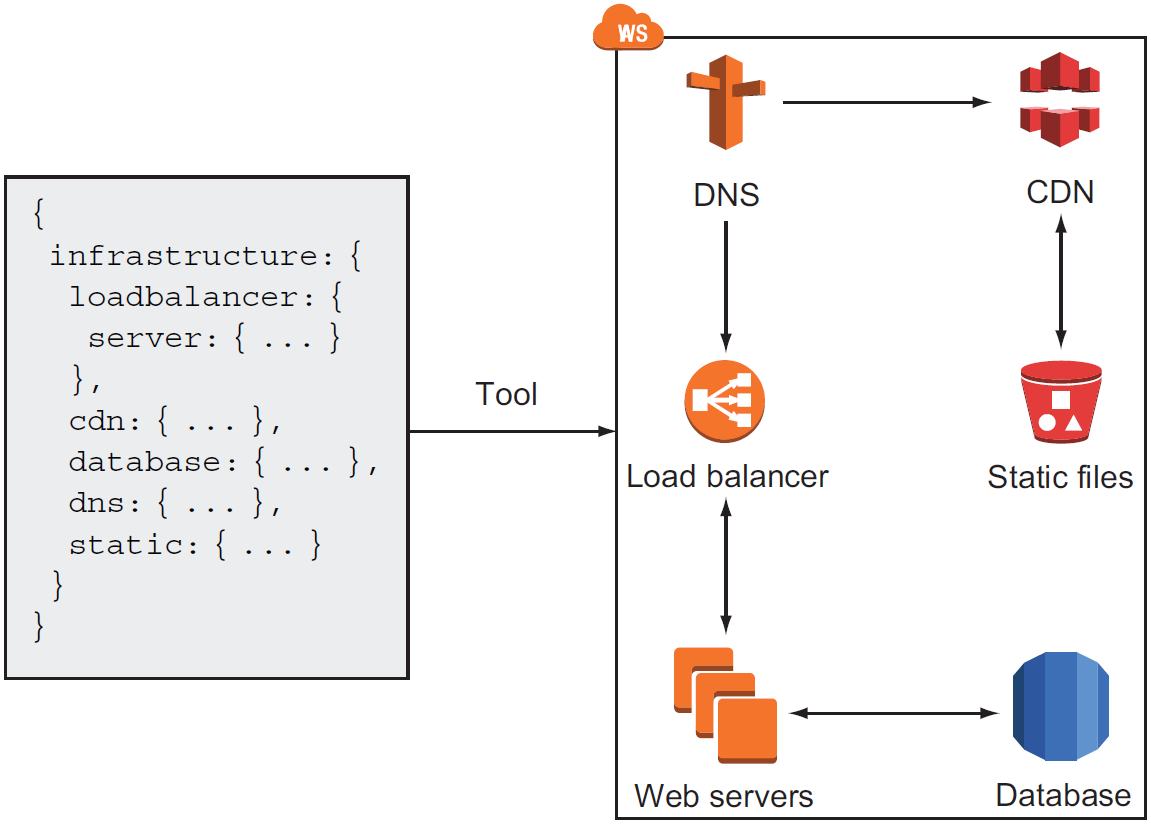
\includegraphics[width=\textwidth]{imgs/aws_blueprint.PNG}
\end{frame}

\begin{frame}{Creating an infrastructure}
    Infrastructure as code
Infrastructure as code describes the idea of using a high-level programming language to
control IT systems. In software development tools like automated tests, code repositories,
and build servers are increasing the quality of software engineering. If your infrastructure
can be treated as code, you can apply the same techniques to infrastructure
code that you do to your application code. In the end, you’ll improve the quality of
your infrastructure by using automated tests, code repositories, and build servers.
WARNING Don’t mix up the terms infrastructure as code and infrastructure as a
service (IaaS)! IaaS means renting servers, storage, and network with a pay-peruse
pricing model.

If you want to use cloud advantages like scaling the number of servers depending on
the current load or building a highly available infrastructure, you’ll need to start new
virtual servers several times a day. On top of that, the number of virtual servers you’ll
have to supply with updates will grow. The steps required to deploy an application
don’t change, but as figure 5.1 shows, you need to perform them on multiple servers.
Deploying software manually to a growing number of servers becomes impossible over
time and has a high risk of human failure. This is why we recommend that you automate
the deployment of applications.

A simple but powerful and flexible way of automating application deployment is to
run a script on server startup. To go from a plain OS to a fully installed and configured
server, you need to follow these three steps:
1 Start a plain virtual server containing just an OS.
2 Execute a script at the end of the boot process.
3 Install and configure your applications with the help of a script.
\end{frame}

\begin{frame}{Service categorization}
Main service categories
\i Compute services, computing power and memory (e.g., virtual servers)
\i App services, solutions for common use cases (message queues, topics, and searching)
\i Deployment and administration, grant/revoke access, monitor servers, deploy applications.
\i Storage, collect and persist data
\i Networking, define private networks, DNS, etc.
\end{frame}

\begin{frame}{Cloud providers}
    Comparing alternatives
AWS isn’t the only cloud computing provider. Microsoft and Google have cloud offerings
as well.
OpenStack is different because it’s open source and developed by more than 200
companies including IBM, HP, and Rackspace. Each of these companies uses Open-
Stack to operate its own cloud offerings, sometimes with closed source add-ons. You
could run your own cloud based on OpenStack, but you would lose most of the benefits
outlined in section 1.3.
Comparing cloud providers isn’t easy, because open standards are mostly missing.
Functionality like virtual networks and message queuing are realized differently. If you
know what features you need, you can compare the details and make your decision.
\end{frame}

\begin{frame}{Data pipeline on AWS cloud}
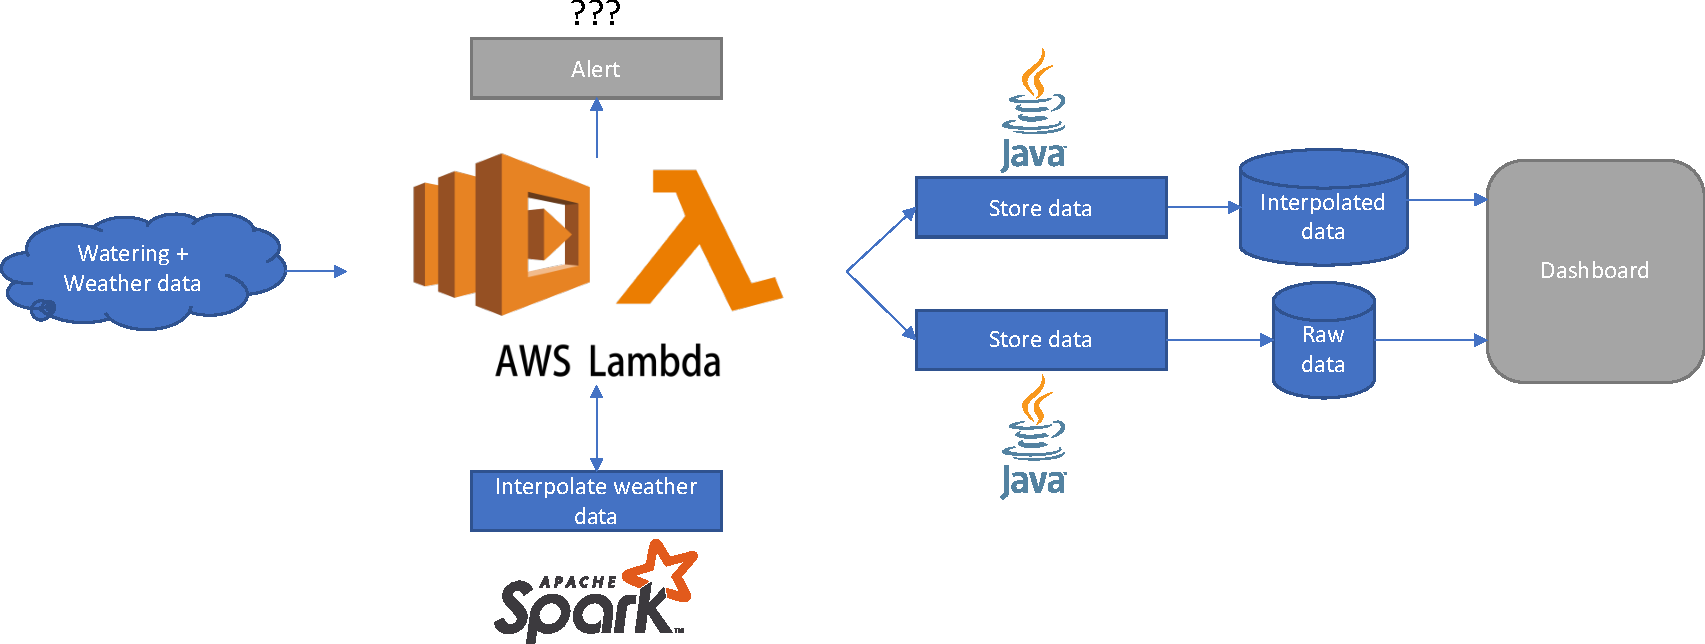
\includegraphics[width=\linewidth]{imgs/pipeline_aws.pdf}
\end{frame}

\ssec{Authentication and authorization}
\begin{frame}[fragile,allowframebreaks]{AWS - Identity and Access Management}

\textbf{Identity and Access Management (IAM)}
\i web service that controls access to AWS resources
\i IAM controls who is \textit{authenticated} and \textit{authorized} to use resources

\textbf{User}
\i unique identity recognized by AWS services and applications
\si individual, system, or application accessing AWS services
\i similar to user in an operating system like Windows or UNIX

After the account creation
\i begin with a single sign-in identity that has complete access
to all AWS services and resources in the account
\i i.e., a \lstinline{root user}
\i do not use the root user for your everyday tasks, even the administrative ones
\i use the root user only to create your first IAM user
\i specify permissions to control which operations a user can perform

What can a user do?
\i place requests to web services such as Amazon S3 and Amazon EC2
\i If permitted, a user has access to all of the resources under the AWS account
\i sers can make requests to AWS services using security credentials
\i \textbf{Explicit} permissions govern a user's ability to call AWS services

\textbf{IAM role}
\i set of permissions for making AWS service requests
\i trusted entities (e.g., such as IAM users) assume roles
\si \textbf{not} associated with a specific user or group
\i delegate access with defined permissions to trusted entities without having to share long-term access keys
\i there is no limit to the number of IAM roles you can assume

Role vs user
\i user has permanent long-term credentials and is used to directly interact with AWS services
\i role does not have any credentials and cannot make direct requests to AWS services
\i IAM roles are meant to be assumed by authorized entities, such as IAM users, applications, or an AWS service such as EC2.

\textbf{Policy}
\i an object in AWS that, when associated with an identity or resource, defines their permissions
\i AWS evaluates these policies when an IAM principal (user or role) makes a request
\i Permissions in the policies determine whether the request is allowed or denied
\i You manage access in AWS by creating policies and attaching them to IAM identities (users, groups of users, or roles)
\i six types of policies (listed in order of frequency)
\si Identity-based policies, grant permissions to an identity.
\si Resource-based policies, e.g. resource-based policies are Amazon S3 bucket policies
\si Permissions boundaries, maximum permissions that the identity-based policies can grant to an entity
\si Service control policy (SCP), maximum permissions for members of an organization or organizational unit (OU)
\si Access control lists (ACLs), which accounts can access the resource to which the ACL is attached.
\si Session policies, limit the permissions that the role or user's identity-based policies grant to the session
\end{frame}

\begin{frame}[fragile,allowframebreaks]{AWS CLI and authentication}
We will mainly refer to the CLI interface
\begin{lstlisting}
Synopsis
********
   aws [options] <command> <subcommand> [parameters]

Description
***********
A unified tool to manage your AWS services.
\end{lstlisting}

First of all it is necessary to install the CLI (version 2)
\i See {\footnotesize \url{https://docs.aws.amazon.com/cli/latest/userguide/install-cliv2.html}}

\framebreak
This is your AWS account

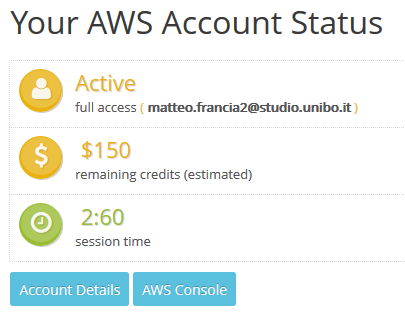
\includegraphics[scale=.5]{imgs/aws_account.PNG}

\framebreak
Click on ``Account Details'' to get your secrets

\i Copy the content into the file \lstinline{~/.aws/configure}
\i \textbf{All examples assume that you have setup your credentials in the credentials file}
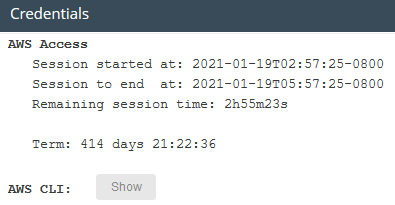
\includegraphics[scale=.5]{imgs/aws_account1.PNG}

\framebreak
Run \lstinline{aws configure}
\i Confirm \lstinline{AWS Access Key ID}
\i Confirm \lstinline{AWS Secret Access Key}
\i Set \lstinline{Default region name} to \lstinline{us-east-1}
\i Set \lstinline{Default output format} to \lstinline{json} 

It is also possible to configure an AWS profile
\i A (named) profile is a collection of settings and credentials
\i If profile is specified, its settings and credentials are used to run a command
\i When no profile is explicitly referenced, use ``default'' 
\si \textbf{We stick to ``default''}

\end{frame}

\ssec{NoSQL}
\begin{frame}[fragile,allowframebreaks]{AWS - NoSQL with DynamoDB}

The following are the basic DynamoDB components:

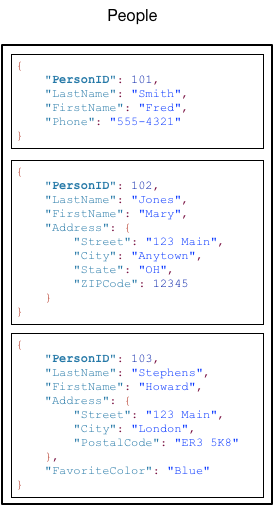
\includegraphics[height=\textheight]{imgs/HowItWorksPeople.png}

\textbf{Tables}
\i a collection of (data) items
\i e.g., example table called People

\textbf{Items}
\i a group of attributes that is uniquely identifiable among all others
\i Each table contains zero or more items
\si no limit to the number of items you can store in a table.
\i Items tuples in other database systems
\si In the People table, each item represents a person. 
\i Each item in the table has a unique identifier, or primary key
\si In the People table, the primary key consists of one attribute (PersonID)

\textbf{Attributes} 
\i a fundamental data element that is not broken down any further
\i e.g., an item in the People table contains attributes PersonID, LastName, FirstName
\i Most of the attributes are scalar (have only one value)
\si Strings and numbers are common examples of scalars
\i Some of the items have a nested attribute (Address)
\si up to 32 levels deep

\textbf{Schemaless}
\i Other than the primary key, the People table is schemaless
\i neither the attributes nor their data types need to be defined beforehand
\i Each item can have its own distinct attributes.

\textbf{Primary Key}
\i To create a table, you must specify the primary key of the table
\i The primary key uniquely identifies each item in the table, 
\si no two items can have the same key.

Two types of primary keys
\i Partition key: a simple primary key, composed of one attribute known as the partition key
\si key values as inputs to an internal hash function
\si The hash function determines the partition (physical storage internal to DynamoDB) in which the item will be stored
\si access any item in the People table directly by providing the PersonId

\i composite primary key: Partition key and sort key (two attributes)
\si first attribute is the partition key
\si second attribute is the sort key
\si items in same partition key value are stored together, in sorted order by sort key

\textbf{Secondary Indexes}
\i one or more secondary indexes per table
\i query data using an alternate key (additionally to queries against primary key) 
\i indexes are automatically maintained on add, update, or delete

Two types of indexes
\i \textbf{Global secondary} has partition and sort keys different from those on table
\i \textbf{Local secondary} has the same partition key but a different sort key
\i Each table has a quota of 20 global and 5 local indexes

How do we shape the schema?
\i \url{https://cloud.google.com/bigtable/docs/schema-design}

\begin{lstlisting}
$ aws dynamodb create-table \
    --table-name soil-humidity \
    --attribute-definitions AttributeName=field,AttributeType=S AttributeName=timestamp,AttributeType=S \
    --key-schema AttributeName=field,KeyType=HASH AttributeName=timestamp,KeyType=RANGE \
    --provisioned-throughput ReadCapacityUnits=1,WriteCapacityUnits=1
    
$ aws dynamodb create-table \
    --table-name interpolate-soil-humidity \
    --attribute-definitions AttributeName=field,AttributeType=S AttributeName=timestamp,AttributeType=S \
    --key-schema AttributeName=field,KeyType=HASH AttributeName=timestamp,KeyType=RANGE \
    --provisioned-throughput ReadCapacityUnits=1,WriteCapacityUnits=1
\end{lstlisting}

Amazon DynamoDB is available in multiple AWS Regions around the world. Each Region is independent and isolated from other AWS Regions. For example, if you have a table called People in the us-east-2 Region and another table named People in the us-west-2 Region, these are considered two entirely separate tables. For a list of all the AWS Regions in which DynamoDB is available, see AWS Regions and Endpoints in the Amazon Web Services General Reference.

Every AWS Region consists of multiple distinct locations called Availability Zones. Each Availability Zone is isolated from failures in other Availability Zones, and provides inexpensive, low-latency network connectivity to other Availability Zones in the same Region. This allows rapid replication of your data among multiple Availability Zones in a Region.

When your application writes data to a DynamoDB table and receives an HTTP 200 response (OK), the write has occurred and is durable. The data is eventually consistent across all storage locations, usually within one second or less.

DynamoDB supports eventually consistent and strongly consistent reads.

Eventually Consistent Reads

When you read data from a DynamoDB table, the response might not reflect the results of a recently completed write operation. The response might include some stale data. If you repeat your read request after a short time, the response should return the latest data.

Strongly Consistent Reads

When you request a strongly consistent read, DynamoDB returns a response with the most up-to-date data, reflecting the updates from all prior write operations that were successful. However, this consistency comes with some disadvantages:

    A strongly consistent read might not be available if there is a network delay or outage. In this case, DynamoDB may return a server error (HTTP 500).

    Strongly consistent reads may have higher latency than eventually consistent reads.

    Strongly consistent reads are not supported on global secondary indexes.

    Strongly consistent reads use more throughput capacity than eventually consistent reads. For details, see Read/Write Capacity Mode

Note

DynamoDB uses eventually consistent reads, unless you specify otherwise. Read operations (such as GetItem, Query, and Scan) provide a ConsistentRead parameter. If you set this parameter to true, DynamoDB uses strongly consistent reads during the operation.


If you choose provisioned mode, you specify the number of reads and writes per second that you require for your application. You can use auto scaling to adjust your table’s provisioned capacity automatically in response to traffic changes. This helps you govern your DynamoDB use to stay at or below a defined request rate in order to obtain cost predictability.

Provisioned mode is a good option if any of the following are true:

    You have predictable application traffic.

    You run applications whose traffic is consistent or ramps gradually.

    You can forecast capacity requirements to control costs.



Read Capacity Units and Write Capacity Units

For provisioned mode tables, you specify throughput capacity in terms of read capacity units (RCUs) and write capacity units (WCUs):

    One read capacity unit represents one strongly consistent read per second, or two eventually consistent reads per second, for an item up to 4 KB in size. Transactional read requests require two read capacity units to perform one read per second for items up to 4 KB. If you need to read an item that is larger than 4 KB, DynamoDB must consume additional read capacity units. The total number of read capacity units required depends on the item size, and whether you want an eventually consistent or strongly consistent read. For example, if your item size is 8 KB, you require 2 read capacity units to sustain one strongly consistent read per second, 1 read capacity unit if you choose eventually consistent reads, or 4 read capacity units for a transactional read request. For more information, see Capacity Unit Consumption for Reads.

Note

To learn more about DynamoDB read consistency models, see Read Consistency.

One write capacity unit represents one write per second for an item up to 1 KB in size. If you need to write an item that is larger than 1 KB, DynamoDB must consume additional write capacity units. Transactional write requests require 2 write capacity units to perform one write per second for items up to 1 KB. The total number of write capacity units required depends on the item size. For example, if your item size is 2 KB, you require 2 write capacity units to sustain one write request per second or 4 write capacity units for a transactional write request. For more information, see Capacity Unit Consumption for Writes.



Putting data

\begin{lstlisting}
$ aws dynamodb create-table \
    --table-name soil-humidity \
    --attribute-definitions AttributeName=field,AttributeType=S AttributeName=timestamp,AttributeType=S \
    --key-schema AttributeName=field,KeyType=HASH AttributeName=timestamp,KeyType=RANGE \
    --provisioned-throughput ReadCapacityUnits=1,WriteCapacityUnits=1

$ aws dynamodb create-table \
    --table-name interpolate-soil-humidity \
    --attribute-definitions AttributeName=field,AttributeType=S AttributeName=timestamp,AttributeType=S \
    --key-schema AttributeName=field,KeyType=HASH AttributeName=timestamp,KeyType=RANGE \
    --provisioned-throughput ReadCapacityUnits=1,WriteCapacityUnits=1

$ aws dynamodb delete-table --table-name soil-humidity

$ aws dynamodb delete-table --table-name interpolate-soil-humidity

$ aws dynamodb list-tables

$ aws dynamodb put-item \
    --table-name soil-humidity \
    --item \
    '{"field": {"S": "field-01"}, "timestamp": {"S": "1611226870"}, "xx": {"N": "0"}, "yy": {"N": "-20"}, "value": {"N": "-17"}}'

$ aws dynamodb put-item \
    --table-name soil-humidity \
    --item \
    '{"field": {"S": "field-01"}, "timestamp": {"N": "1611226880"}, "xx": {"S": "0"}, "yy": {"S": "-20"}, "value": {"S": "-20"}}'
    
$ aws kinesis put-record --stream-name events --partition-key soilhumidity --cli-binary-format raw-in-base64-out --data \
    '{"field": "field-01", "timestamp": "1611226890", "xx": "0", "yy": "-20", "value": "-23", "message": "Hello from AWS CLI!"}'

$ aws kinesis put-record --stream-name events --partition-key soilhumidity --cli-binary-format raw-in-base64-out --data \
    '{"field": "field-01", "timestamp": "1611226900", "xx": "0", "yy": "-20", "value": "-26", "message": "Hello from AWS CLI!"}'
\end{lstlisting}



The Query operation in Amazon DynamoDB finds items based on primary key values.

You must provide the name of the partition key attribute and a single value for that attribute. Query returns all items with that partition key value. Optionally, you can provide a sort key attribute and use a comparison operator to refine the search results. 

To specify the search criteria, you use a key condition expression—a string that determines the items to be read from the table or index.

You must specify the partition key name and value as an equality condition.

You can optionally provide a second condition for the sort key (if present). The sort key condition must use one of the following comparison operators:

    a = b — true if the attribute a is equal to the value b

    a < b — true if a is less than b

    a <= b — true if a is less than or equal to b

    a > b — true if a is greater than b

    a >= b — true if a is greater than or equal to b

    a BETWEEN b AND c — true if a is greater than or equal to b, and less than or equal to c.

The following function is also supported:

    begins_with (a, substr)— true if the value of attribute a begins with a particular substring.



\begin{lstlisting}
$ aws dynamodb query \
    --table-name soil-humidity \
    --key-condition-expression "field = :n" \
    --expression-attribute-values '{":n":{"S":"field-01"}}'

$ aws dynamodb query \
    --table-name soil-humidity \
    --key-condition-expression "field = :n" \
    --expression-attribute-values '{":n":{"S":"field-02"}}'
    
aws dynamodb delete-table --table-name soil-humidity

aws dynamodb delete-table --table-name interpolate-soil-humidity

aws dynamodb create-table \
  --table-name soil-humidity \
  --attribute-definitions AttributeName=field,AttributeType=S AttributeName=timestamp,AttributeType=S \
  --key-schema AttributeName=field,KeyType=HASH AttributeName=timestamp,KeyType=RANGE \
  --provisioned-throughput ReadCapacityUnits=1,WriteCapacityUnits=1

aws dynamodb create-table \
  --table-name interpolate-soil-humidity \
  --attribute-definitions AttributeName=field,AttributeType=S AttributeName=sensorid,AttributeType=S \
  --key-schema AttributeName=field,KeyType=HASH AttributeName=sensorid,KeyType=RANGE \
  --provisioned-throughput ReadCapacityUnits=1,WriteCapacityUnits=1

aws dynamodb query \
  --table-name soil-humidity \
  --key-condition-expression "field = :n" \
  --expression-attribute-values '{":n":{"S":"field-01"}}'

aws dynamodb query \
  --table-name soil-humidity \
  --key-condition-expression "field = :n" \
  --expression-attribute-values '{":n":{"S":"field-02"}}'

aws dynamodb query \
  --table-name soil-humidity \
  --key-condition-expression "field = :n" \
  --expression-attribute-values '{":n":{"S":"field-00"}}'

aws dynamodb query \
  --table-name interpolate-soil-humidity \
  --key-condition-expression "field = :n" \
  --expression-attribute-values '{":n":{"S":"field-00"}}'
\end{lstlisting}

Filter Expressions for Query

If you need to further refine the Query results, you can optionally provide a filter expression. A filter expression determines which items within the Query results should be returned to you. All of the other results are discarded.

A filter expression is applied after a Query finishes, but before the results are returned. Therefore, a Query consumes the same amount of read capacity, regardless of whether a filter expression is present.

A Query operation can retrieve a maximum of 1 MB of data. This limit applies before the filter expression is evaluated.

A filter expression cannot contain partition key or sort key attributes. You need to specify those attributes in the key condition expression, not the filter expression.

The syntax for a filter expression is identical to that of a condition expression. Filter expressions can use the same comparators, functions, and logical operators as a condition expression, with the addition of the not-equals operator (<>). For more information, see Condition Expressions.

Example

The following AWS CLI example queries the Thread table for a particular ForumName (partition key) and Subject (sort key). Of the items that are found, only the most popular discussion threads are returned—in other words, only those threads with more than a certain number of Views. 

\begin{lstlisting}

$ aws dynamodb query \
    --table-name Thread \
    --key-condition-expression "ForumName = :fn and Subject = :sub" \
    --filter-expression "#v >= :num" \
    --expression-attribute-names '{"#v": "Views"}' \
    --expression-attribute-values file://values.json
 
\end{lstlisting}
The arguments for --expression-attribute-values are stored in the values.json file. 
\begin{lstlisting}
{
    ":fn":{"S":"Amazon DynamoDB"},
    ":sub":{"S":"DynamoDB Thread 1"},
    ":num":{"N":"3"}
}
\end{lstlisting}

\end{frame}

\ssec{Event streams}
\begin{frame}[fragile,allowframebreaks]{AWS - Event streams with Kinesis}
Creating a Kinesis stream

Kinesis Data Stream
\i A Kinesis data stream is a set of shards. 
\i Each shard has a sequence of data records. 
\i Each data record has a sequence number that is assigned by Kinesis Data Streams.

Data Record
\i unit of data stored in a Kinesis data stream. 
\i Data records are composed of a sequence number, a partition key, and a data blob
\i Kinesis Data Streams does not inspect, interpret, or change the data in the blob in any way. 
\i A data blob can be up to 1 MB.

Retention Period
\i the length of time that data records are accessible after they are added to the stream
\i A stream’s retention period is set to a default of 24 hours after creation.
\i Additional charges apply for streams with a retention period set to more than 24 hours. For more information, see Amazon Kinesis Data Streams Pricing

Producer
\i Producers put records into Amazon Kinesis Data Streams

Consumer
\i Get and process records from Amazon Kinesis Data Streams
\i Also known as Amazon Kinesis Data Streams Application

Two types of consumers that you can develop
\i shared fan-out consumers 
\i enhanced fan-out consumers
\i The output of a Kinesis Data Streams application can be input for another stream, enabling you to create complex topologies that process data in real time. 
\i An application can also send data to a variety of other AWS services. 
\i There can be multiple applications for one stream, and each application can consume data from the stream independently and concurrently.

Shard
\i sequence of data records in a stream
\i A stream is composed of one or more shards, each of which provides a fixed unit of capacity. 
\i Each shard can support up to 5 transactions per second for reads, up to a maximum total data read rate of 2 MB per second and up to 1,000 records per second for writes, up to a maximum total data write rate of 1 MB per second (including partition keys). The data capacity of your stream is a function of the number of shards that you specify for the stream. The total capacity of the stream is the sum of the capacities of its shards.

If your data rate increases, you can increase or decrease the number of shards allocated to your stream. For more information, see Resharding a Stream.


Partition Key
\i A partition key is used to group data by shard within a stream. Kinesis Data Streams segregates the data records belonging to a stream into multiple shards. It uses the partition key that is associated with each data record to determine which shard a given data record belongs to. Partition keys are Unicode strings, with a maximum length limit of 256 characters for each key. An MD5 hash function is used to map partition keys to 128-bit integer values and to map associated data records to shards using the hash key ranges of the shards. When an application puts data into a stream, it must specify a partition key. 

\begin{lstlisting}
$ aws kinesis create-stream --stream-name events --shard-count 2

$ aws kinesis delete-stream --stream-name events

$ aws kinesis describe-stream --stream-name events

$ aws kinesis get-shard-iterator --stream-name=events \
    --shard-id=shardId-000000000000 --shard-iterator-type=TRIM_HORIZON
{
    "ShardIterator": "iterator-id-00"
}

$ aws kinesis get-records --shard-iterator "iterator-id-00"
{
    "Records": [],
    "NextShardIterator": "iterator-id-01",
    "MillisBehindLatest": 0
}

$ aws kinesis get-records --shard-iterator  "iterator-id-01"
{
    "Records": [],
    "NextShardIterator": "iterator-id-02",
    "MillisBehindLatest": 0
}
\end{lstlisting}

Created a stream with two shards
\i events sent will be written to one or either of the two shards
\i stream processing apps read events from all shards
\i Status {\footnotesize\url{https://console.aws.amazon.com/kinesis/home?region=us-east-1#/streams/list}}

We specified that the shard iterator should be of type TRIM\_HORIZON. This is AWS jargon
for the oldest events in the shard that have not yet been trimmed—expired for
being too old. At the time of writing, records are trimmed from a Kinesis stream after
a fixed period of 24 hours

\framebreak

Creating the producer using Amazon SDK
\i need to be able to send events to it from all our various client applications
\si E.g., Producer in Python using Amazon SDK (boto3)
\end{frame}

\ssec{Serverless}
\begin{frame}{Going serverless}
Amazon AWS Lambda as a case study
\i Execute code in a massively parallelized way in response to events
\i Elastic Compute Cloud (EC2) servers run the code
\si E.g., Linux server with distribution
Amazon Linux
\i See also Microsoft Azure Functions, IBM Bluemix, Google Cloud Functions

AWS lambda
\i The Lambda runtime invokes a lambda function multiple times in parallel
\i Invocation supports push/pull event models
\i \textbf{Lambda function}: code + configuration + dependencies
\i Compute service that executes code written in JavaScript/Python/C\#/Java
\i Source code (JARs or DLLs) is zipped up and deployed to a container

In AWS, every Lambda function is a granular service
\i Inputs and outputs should be clearly defined (i.e., a clear interface)
\si Similar to the compute-as-glue architecture we described previously
\i Make sure your function follows the single-responsibility principle
\i Make the function idempotent (i.e., given an input produce the same output)
\i Clearly define an interface for the function
\si Make sure inputs and outputs are clearly stated
\i Function are black-boxes
\si consumer should not have to know how it works

\end{frame}

\begin{frame}[fragile,allowframebreaks]{AWS - Serverless with Lambda}
AWS Lambda is a compute service that lets you run code without provisioning or managing servers.
Lambda runs your code only when needed and scales automatically, from a few requests per day
to thousands per second. You pay only for the compute time that you consume—there is no charge
when your code is not running. With Lambda, you can run code for virtually any type of application or
backend service, all with zero administration. Lambda runs your code on a high-availability compute
infrastructure and performs all of the administration of the compute resources, including server and
operating system maintenance, capacity provisioning and automatic scaling, code monitoring and
logging.

When using Lambda, you are responsible only for your code. Lambda manages the compute fleet that
offers a balance of memory, CPU, network, and other resources. This is in exchange for flexibility, which
means you cannot log in to compute instances, or customize the operating system on provided runtimes.
These constraints enable Lambda to perform operational and administrative activities on your behalf,
including provisioning capacity, monitoring fleet health, applying security patches, deploying your code,
and monitoring and logging your Lambda functions.

Create a function
\i \url{https://console.aws.amazon.com/lambda/home?region=us-east-1#/functions}

The following "create-function" example creates a Lambda function
named "my-function".
\begin{lstlisting}
$ aws iam create-role --role-name lambda-execute

$ aws iam attach-role-policy \
    --policy-arn arn:aws:iam::aws:policy/service-role/AWSLambdaKinesisExecutionRole --role-name lambda-execute

$ aws iam attach-role-policy \
    --policy-arn arn:aws:iam::aws:policy/AWSLambdaInvocation-DynamoDB --role-name lambda-execute

$ aws iam attach-role-policy \
    --policy-arn arn:aws:iam::aws:policy/service-role/AWSLambdaDynamoDBExecutionRole --role-name lambda-execute

$ aws iam attach-role-policy \
    --policy-arn arn:aws:iam::aws:policy/AmazonDynamoDBFullAccess --role-name lambda-execute

$ aws iam attach-role-policy \
    --policy-arn arn:aws:iam::aws:policy/AmazonDynamoDBFullAccesswithDataPipeline --role-name lambda-execute

$ aws lambda create-function \
    --function-name my-function \
    --runtime nodejs10.x \
    --zip-file fileb://my-function.zip \
    --handler my-function.handler \
    --role rolename
\end{lstlisting}
\i \lstinline{zip-file} deployment package that contains code and dependencies
\i \lstinline{handler} name of the method that Lambda calls to execute your function

\begin{lstlisting}
import boto3
import time
def lambda_handler(event, context):
    client = boto3.resource('dynamodb') # create dynamodb resource
    table = client.Table("soil-humidity") # search for dynamoDB table
    table.put_item(Item={
            "field": "field-01", # partition key
            "timestamp": str(int(time.time())), # sort key
            "xx": "0", "yy": "-20", "value": "-25",
            "message": "Hello from Lambda!"})
\end{lstlisting}
\end{frame}

% \ssec{Computing}
% \begin{frame}[fragile,allowframebreaks]{AWS - Computing with EC2}

% Amazon Elastic Compute Cloud (Amazon EC2) provides scalable computing capacity in the Amazon Web
% Services (AWS) Cloud. Using Amazon EC2 eliminates your need to invest in hardware up front, so you
% can develop and deploy applications faster. You can use Amazon EC2 to launch as many or as few virtual
% servers as you need, configure security and networking, and manage storage. Amazon EC2 enables you
% to scale up or down to handle changes in requirements or spikes in popularity, reducing your need to
% forecast traffic

% Instances and AMIs
% An Amazon Machine Image (AMI) is a template that contains a software configuration (for example, an
% operating system, an application server, and applications). From an AMI, you launch an instance, which is a copy of the AMI running as a virtual server in the cloud. You can launch multiple instances of an AMI, as
% shown in the following figure.

% Instances
% An instance is a virtual server in the cloud. Its configuration at launch is a copy of the AMI that you
% specified when you launched the instance.
% You can launch different types of instances from a single AMI. An instance type essentially determines
% the hardware of the host computer used for your instance. Each instance type offers different compute
% and memory capabilities. Select an instance type based on the amount of memory and computing power
% that you need for the application or software that you plan to run on the instance. For more information
% about the hardware specifications for each Amazon EC2 instance type, see Amazon EC2 Instance Types.
% After you launch an instance, it looks like a traditional host, and you can interact with it as you would any
% computer. You have complete control of your instances; you can use sudo to run commands that require
% root privileges.
% Your AWS account has a limit on the number of instances that you can have running. For more
% information about this limit, and how to request an increase, see How many instances can I run in
% Amazon EC2 in the Amazon EC2 General FAQ.
% Storage for your instance
% The root device for your instance contains the image used to boot the instance. For more information,
% see Amazon EC2 root device volume (p. 21).
% Your instance may include local storage volumes, known as instance store volumes, which you
% can configure at launch time with block device mapping. For more information, see Block device
% mapping (p. 1283). After these volumes have been added to and mapped on your instance, they are
% available for you to mount and use. If your instance fails, or if your instance is stopped or terminated,
% the data on these volumes is lost; therefore, these volumes are best used for temporary data. To keep
% important data safe, you should use a replication strategy across multiple instances, or store your
% persistent data in Amazon S3 or Amazon EBS volumes

% Regions and Zones
% Amazon EC2 is hosted in multiple locations world-wide. These locations are composed of Regions,
% Availability Zones, Local Zones, AWS Outposts, and Wavelength Zones. Each Region is a separate
% geographic area.
% • Availability Zones are multiple, isolated locations within each Region.
% • Local Zones provide you the ability to place resources, such as compute and storage, in multiple
% locations closer to your end users.
% • AWS Outposts brings native AWS services, infrastructure, and operating models to virtually any data
% center, co-location space, or on-premises facility.
% • Wavelength Zones allow developers to build applications that deliver ultra-low latencies to 5G devices
% and end users. Wavelength deploys standard AWS compute and storage services to the edge of
% telecommunication carriers' 5G networks.

% Available Regions
% Your account determines the Regions that are available to you.
% • An AWS account provides multiple Regions so that you can launch Amazon EC2 instances in locations
% that meet your requirements. For example, you might want to launch instances in Europe to be closer
% to your European customers or to meet legal requirements.
% • An AWS GovCloud (US-West) account provides access to the AWS GovCloud (US-West) Region and the
% AWS GovCloud (US-East) Region. For more information, see AWS GovCloud (US).
% • An Amazon AWS (China) account provides access to the Beijing and Ningxia Regions only. For more
% information, see AWS in China.

% Use the describe-regions command as follows to describe the Regions that are enabled for your
% account.

% Each Region has multiple, isolated locations known as Availability Zones. When you launch an instance,
% you can select an Availability Zone or let us choose one for you. If you distribute your instances across
% multiple Availability Zones and one instance fails, you can design your application so that an instance in
% another Availability Zone can handle requests.
% The following diagram illustrates multiple Availability Zones in an AWS Region.
% You can also use Elastic IP addresses to mask the failure of an instance in one Availability Zone by rapidly
% remapping the address to an instance in another Availability Zone. For more information, see Elastic IP
% addresses (p. 821).
% An Availability Zone is represented by a Region code followed by a letter identifier; for example,
% us-east-1a. To ensure that resources are distributed across the Availability Zones for a Region, we
% independently map Availability Zones to names for each AWS account. For example, the Availability Zone
% us-east-1a for your AWS account might not be the same location as us-east-1a for another AWS
% account.
% To coordinate Availability Zones across accounts, you must use the AZ ID, which is a unique and
% consistent identifier for an Availability Zone. For example, use1-az1 is an AZ ID for the us-east-1
% Region and it has the same location in every AWS account.

% When you launch an instance, select a Region that puts your instances closer to specific customers, or
% meets the legal or other requirements that you have. By launching your instances in separate Availability
% Zones, you can protect your applications from the failure of a single location.
% When you launch an instance, you can optionally specify an Availability Zone in the Region that you are
% using. If you do not specify an Availability Zone, we select an Availability Zone for you. When you launch
% your initial instances, we recommend that you accept the default Availability Zone, because this allows us
% to select the best Availability Zone for you based on system health and available capacity. If you launch
% additional instances, specify a Zone only if your new instances must be close to, or separated from, your
% running instances.

% Amazon EC2 root device volume
% When you launch an instance, the root device volume contains the image used to boot the instance. When
% we introduced Amazon EC2, all AMIs were backed by Amazon EC2 instance store, which means the root
% device for an instance launched from the AMI is an instance store volume created from a template stored
% in Amazon S3. After we introduced Amazon EBS, we introduced AMIs that are backed by Amazon EBS.
% This means that the root device for an instance launched from the AMI is an Amazon EBS volume created
% from an Amazon EBS snapshot.
% You can choose between AMIs backed by Amazon EC2 instance store and AMIs backed by Amazon EBS.
% We recommend that you use AMIs backed by Amazon EBS, because they launch faster and use persistent
% storage.
% Important
% Only the following instance types support an instance store volume as the root device: C3, D2,
% G2, I2, M3, and R3.
% For more information about the device names Amazon EC2 uses for your root volumes, see Name devices
% on Linux instances (p. 1281).
% Contents
% • Root device storage concepts (p. 21)
% • Choose an AMI by root device type (p. 23)
% • Determine the root device type of your instance (p. 23)
% • Change the root volume to persist (p. 24)
% • Change the initial size of the root volume (p. 26)
% Root device storage concepts
% You can launch an instance from either an instance store-backed AMI or an Amazon EBS-backed AMI.
% The description of an AMI includes which type of AMI it is; you'll see the root device referred to in some
% places as either ebs (for Amazon EBS-backed) or instance store (for instance store-backed). This is
% important because there are significant differences between what you can do with each type of AMI. For
% more information about these differences, see Storage for the root device (p. 96).
% Instance store-backed instances
% Instances that use instance stores for the root device automatically have one or more instance store
% volumes available, with one volume serving as the root device volume. When an instance is launched, the
% image that is used to boot the instance is copied to the root volume. Note that you can optionally use
% additional instance store volumes, depending on the instance type.
% Any data on the instance store volumes persists as long as the instance is running, but this data is
% deleted when the instance is terminated (instance store-backed instances do not support the Stop
% action) or if it fails (such as if an underlying drive has issues).

% Create a key pair
% AWS uses public-key cryptography to secure the login information for your instance. A Linux instance has
% no password; you use a key pair to log in to your instance securely. You specify the name of the key pair
% when you launch your instance, then provide the private key when you log in using SSH.
% If you haven't created a key pair already, you can create one using the Amazon EC2 console. Note that
% if you plan to launch instances in multiple Regions, you'll need to create a key pair in each Region. For
% more information about Regions, see Regions and Zones (p. 7).
% You can create a key pair using one of the following methods.

% Create a security group
% Security groups act as a firewall for associated instances, controlling both inbound and outbound traffic
% at the instance level. You must add rules to a security group that enable you to connect to your instance from your IP address using SSH. You can also add rules that allow inbound and outbound HTTP and
% HTTPS access from anywhere.
% Note that if you plan to launch instances in multiple Regions, you'll need to create a security group in
% each Region. For more information about Regions, see Regions and Zones (p. 7).

% If an IAM user wants to launch an EC2 instance, you need to grant the EC2 RunInstances permission to that user. If the EC2 instance should include an instance profile—that is, if applications in the EC2 instance will be able to get temporary security credentials via an IAM role—the user who launches the EC2 instance must also have the IAM PassRole permission. Not only that, but the user might need PassRole permission to associate a specific role with the EC2 instance. If the user doesn’t have PassRole permission, he or she can’t associate a role with the instance during launch. The PassRole permission is a security protection, as we’ll explain in a moment

% \begin{lstlisting}
% $ aws ec2 describe-regions

% $ aws ec2 describe-images --owners amazon --filters "Name=name,Values=amzn*" --query 'sort_by(Images, &CreationDate)[].Name'

% $ aws ssm get-parameters-by-path --path "/aws/service/ami-amazon-linux-latest" --region us-east-1

% $ aws ec2 describe-availability-zones --region us-east-1

% $ aws ec2 create-key-pair --key-name bigdata --output text > ec2key.pem

% $ aws iam list-roles --query "Roles[?RoleName == 'example-role'].[RoleName, Arn]"

% $ aws ec2 run-instances \
%     --image-id resolve:ssm:/aws/service/ami-amazon-linux-latest/amzn2-ami-hvm-x86_64-gp2 \
%     --instance-type t2.micro \
%     --key-name bigdata

% An error occurred (SsmAccessDenied) when calling the RunInstances operation: User: arn:aws:sts::604905954159:assumed-role/vocstartsoft/user307550=matteo.francia2@studio.unibo.it is not authorized to perform: ssm:GetParameters on resource: arn:aws:ssm:us-east-1:604905954159:parameter/aws/service/ami-amazon-linux-latest/amzn2-ami-hvm-x86_64-gp2 with an explicit deny


% $ aws ec2 stop-instances --instance-ids instance_id

% $ aws ec2 start-instances --instance-ids instance_id

% $ aws ec2 terminate-instances --instance-ids instance_id

% ssh -i /path/my-key-pair.pem my-instance-user-name@my-instance-public-dns-name
% \end{lstlisting}
% \end{frame}